\documentclass[a4paper,12pt,final]{article}

\usepackage[italian]{babel}
\usepackage{verbatim}
\usepackage{hyperref}
\usepackage{graphicx}

\begin{document}

\title{Documentazione del client}
\date{2 luglio 2011}
\author{Marco Poletti}

\maketitle

\section*{Introduzione}

Questo documento descrive le varie iterazioni che hanno portato
all'implementazione finale della parte client del progetto Cupido.

\section{Implementazione del cambio di schermata}

La prima iterazione si \`e posta l'obbiettivo di creare la struttura di base
per il cambio di schermata.

Il client in ogni momento mostra un'unica schermata.
La classe che gestisce la schermata ha la possibilit\`a di gestire gli eventi,
sia quelli generati dall'interazione dell'utente utilizzando i vari controlli
grafici visualizzati, sia quelli ricevuti dalla servlet attraverso Comet
(ma questi ultimi verranno implementati solo in una iterazione successiva).

In questa iterazione sono stati aggiunti degli stub per le schermate non
ancora implementate.

\section{Implementazione della grafica di gioco}

In questa iterazione \`e stata implementata la grafica di gioco, comprese
le animazioni per il movimento delle carte sul tavolo, ma senza la logica
necessaria a decidere quando eseguire le varie animazioni.

La classe pi\`u significativa, in relazione a questa iterazione, \`e
\verb@CardsGameWidget@. Questa classe potrebbe essere riutilizzata anche
per altri giochi di carte a due o a quattro giocatori, non dipendendo dalle
regole di Hearts.

\section{Preparazione alla logica di gioco}

In questa iterazione \`e stata creata la struttura necessaria per gestire
i vari stati del gioco. La servlet non era ancora pronta per fornire i servizi
richiesti, quindi in questa iterazione non \`e stata implementata la logica di
gioco, ma si \`e preparato il codice in modo da poterla aggiungere facilmente
in un secondo momento.

Per la logica di gioco, \`e stato usato il pattern \emph{State}; per ogni
stato del gioco \`e stata implementata una classe diversa, per poter gestire
gli eventi in modi differenti, in base allo stato attuale.

Il diagramma degli stati di gioco \`e in figura \ref{fig:stati di gioco}.

\begin{figure}
  \begin{center}
    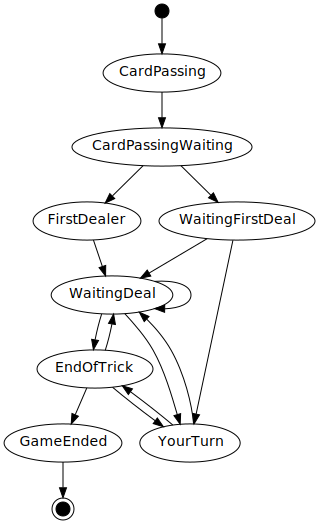
\includegraphics[scale=0.5]{states}
  \end{center}
  \caption{Il diagramma degli stati di gioco}
  \label{fig:stati di gioco}
\end{figure}

In particolare, alla ricezione di una notifica Comet essa viene inoltrata
alla classe che gestisce la schermata attuale.
Molte schermate sono in grado di gestire direttamente questi eventi.

Le schermate di gioco, data la loro complessit\`a, inoltrano tali notifiche
allo stato corrente, in modo da ripartire al meglio il codice fra i vari
stati, per migliorare la manutenibilit\`a del codice.

Non tutti gli stati sono in grado di gestire tutte le notifiche; ad esempio
lo stato \verb@EndOfTrickState@, che visualizza l'animazione con cui le carte
vengono traslate verso il giocatore che ha giocato la carta pi\`u alta, non ha
modo di gestire la notifica \verb@CardPlayed@, con cui la servlet informa il
client che una certa carta \`e stata giocata.

Si \`e quindi resa necessaria la possibilit\`a di rimandare la gestione delle
notifiche ad uno stato successivo. In questo modo, all'arrivo di una notifica,
si prova a farla gestire allo stato corrente; se ci\`o non \`e possibile, tale
notifica viene mantenuta dal gestore degli stati, in una coda, e verr\`a
notificata nuovamente alla prossima transizione di stato, finch\'e non sar\`a
gestita.


\section{Implementazione della logica di gioco e delle schermate rimanenti}

Nel design di massima si \`e cercato di ridurre il carico computazionale
del client, per migliorare le prestazioni, delegando il pi\`u possibile
le computazioni nel backend; per questo motivo, non \`e stato necessario
implementare completamente la logica di gioco, ma solo alcune parti.

A questo punto, la servlet era abbastanza sviluppata da poter comunicare con
il client, e quindi \`e stato possibile implementare la logica di gioco,
compresa appunto l'interazione con la servlet.

Si \`e reso possibile anche lo sviluppo delle rimanenti schermate,
caratterizzate da frequenti comunicazioni con la servlet.


\end{document}
